\chapter{Lecture 16 - Texture}
Texturing is a fundamental technology in computer graphics used to add high levels of visual detail to 3D surfaces without requiring complex geometric modeling.

\begin{definition}
    Texturing is the process of modulating the attributes of vertices, such as color, normals, or transparency, to obtain a specific visual effect.
\end{definition}

During rendering, textures are stored in a specialized memory on the graphics card called Texture RAM. Each texture is a 1D, 2D, or 3D array of \textbf{texels} of the same data type (a texel is the base element, just like a picture is made of pixels). Depending on what the texel represents, a texture can be a color map (RGB), an alpha map (transparency), a normal map (surface orientation: X, Y, Z), or a shininess map (specular coefficients).

The most common form of texturing is \textbf{texture mapping}, where the color attribute is modulated to wrap a 2D image around a 3D object.\par
To tell the computer how to wrap the image, every vertex in a 3D model is assigned coordinates in a 2D "texture space", also known as \textbf{uv space}.

\subsection{UV space}
Every vertex in a 3D mesh is assigned a coordinate (x, v) ranging from 0.0 to 1.0, which corresponds to a specific location on the 2D texture image. During rasterization, these u, v coordinates are interpolated across the face of a triangle so the system knows which part of the image belongs to which pixel. \par
These u, v coordinates can be assigned manually during modeling, precomputed, or generated automatically using projection functions. Different techniques of texture coordinates assignment need to be uses to speed up the texture transfer CPU RAM - Texture RAM. The specific technique to be used depends on the application.\par

\begin{figure}[htbp]
    \centering
    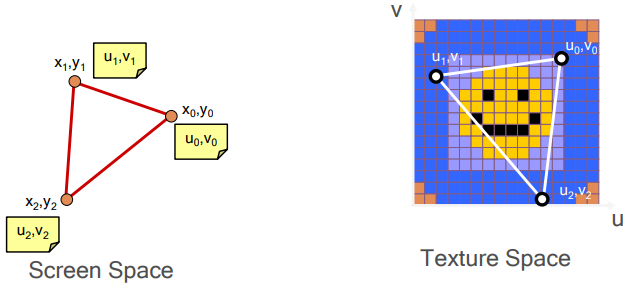
\includegraphics[width=0.5\linewidth]{imgs/lecture16/16.1.png}
    \caption{UV Space}
    \label{fig:16.1}
\end{figure}

Attribute interpolation using Barycentric coordinates and perspective correction is also used here in texturing.

\begin{figure}[htbp]
    \centering
    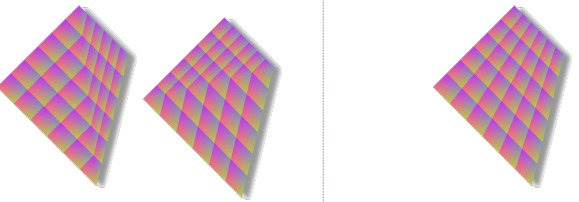
\includegraphics[width=0.4\linewidth]{imgs/lecture16/16.2 attribute interpolation.png}
    \caption{Left without interpolation, right with interpolation}
    \label{fig:16.2}
\end{figure}

\subsection{Texture look up}
When a pixel on the screen does not perfectly align with a texel in the image, the system must perform a texture look-up using filtering techniques:
\begin{itemize}[noitemsep]
    \item \textbf{Magnification} is used when a pixel is larger than a texel. To avoid a "blocky" look, the system uses \textit{nearest filtering} (choosing the closest texel) or \textit{bilinear interpolation} (averaging the closest texels for a smoother look)
    \item \textbf{Minification} is used when a pixel is smaller than a texel. This often causes visual artifacts like aliasing. The standard solution is \textit{mip-mapping}, where the system pre-computes several lower-resolution versions of the texture and chooses the one that best matches the current viewing distance.
\end{itemize}

\begin{figure}[htbp]
    \centering
    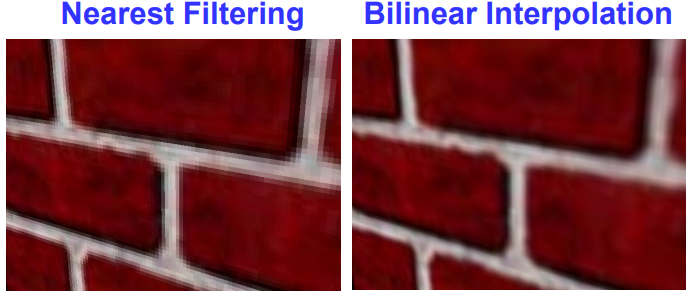
\includegraphics[width=0.3\linewidth]{imgs/lecture16/16.4 magnification.png}
    \caption{Magnification methods comparison}
    \label{fig:16.3}
\end{figure}

\begin{figure}[htbp]
    \centering
    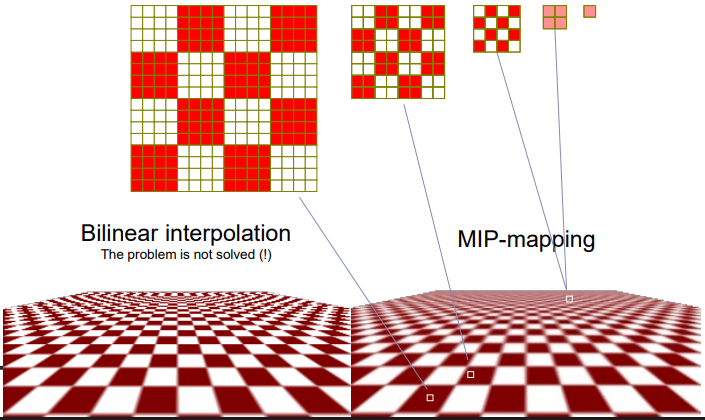
\includegraphics[width=0.5\linewidth]{imgs/lecture16/16.3 mip-mapping.png}
    \caption{Mip-mapping visualized}
    \label{fig:16.4}
\end{figure}

If a vertex is assigned texture coordinates outside the standard range, the system uses one of two modes: 
\begin{itemize}[noitemsep]
    \item \textbf{Clamp mode}, any coordinate less than 0 is treated as 0, and anything greater than 1 is treated as 1, effectively stretching the edge texels
    \item \textbf{Repeat mode}, the integer part of the coordinate is ignored, causing the texture to tile across the surface, which is highly efficient for larger surfaces like brick walls.
\end{itemize}

\subsection{Advanced mapping techniques}
Building on the standard color modulation of texture mapping, the following advanced mapping techniques designed to simulate complex optical effects and intricate surface details. 

\subsubsection{Environmental mapping}
The environmental mapping is used to simulate an object reflecting its surroundings without the high computational cost of full ray tracing. A texture, known as an environment map, captures the colors of the reflected scene. There are two primary methods for applying this:
\begin{itemize}[noitemsep]
    \item \textbf{Sphere mapping}: the technique maps the environment onto a virtual sphere surrounding the object. It uses spherical coordinates derived from the reflection vector to determine which part of the environment is visible from the observer's viewpoint.
    \item \textbf{Cube mapping}: this is often preferred because it provides more uniform sampling than sphere mapping and is easier to generate. The environment is projected onto the six faces of a virtual cube. 
\end{itemize}

\subsubsection{Bump mapping}
Bump mapping is introduced as a way to simulate surface irregularities like wrinkles or bumps. Bump mapping alters the way light hits a surface without modifying its actual 3D geometry. The technique uses a texture (a normal map) to perturb the surface normals of an object. Because lighting calculations depend heavily on surface normals, the light "tricks" the eye into seeing depth and texture on a perfectly flat surface. However, because the geometry is unchanged, the silhouette of the object remains perfectly smooth.

\subsubsection{Displacement mapping}
Displacement mapping is a more advanced alternative to bump mapping that provides a much higher level of realism. Unlike bump mapping, this technique effectively moves the 3D points of the surface during rendering. Because the geometry itself is moved, the silhouette of the model is correctly deformed. This allows for the realistic rendering of very rough surfaces, such as jagged rocks or heavy cratering, that bump mapping cannot convincingly simulate. 

\begin{figure}[htbp]
    \centering
    
    % First row
    \begin{subfigure}{0.45\textwidth}
        \centering
        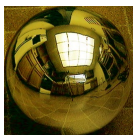
\includegraphics[width=0.4\linewidth]{imgs/lecture16/16.5 sphere mapping.png}
        \caption{Sphere mapping example}
        \label{fig:16.5a}
    \end{subfigure}
    \hfill
    \begin{subfigure}{0.45\textwidth}
        \centering
        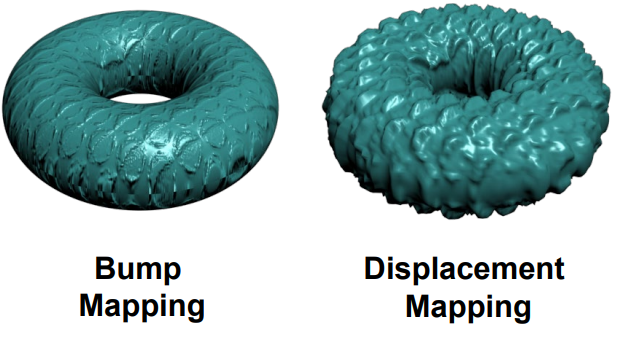
\includegraphics[width=0.8\linewidth]{imgs/lecture16/16.7 bump and displacement mapping.png}
        \caption{Bump mapping and displacement mapping examples}
        \label{fig:16.5b}
    \end{subfigure}

    \vspace{0.5cm}

    % Second row 
    \begin{subfigure}{\textwidth}
        \centering
        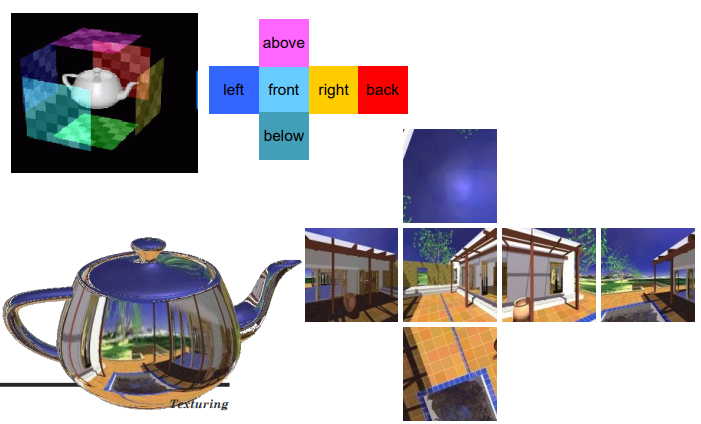
\includegraphics[width=0.7\linewidth]{imgs/lecture16/16.6 cube mapping.png}
        \caption{Cube mapping example}
        \label{fig:16.5c}
    \end{subfigure}

    \caption{Texture techniques}
    \label{fig:16.5}
\end{figure}